%Mid-Year Cadidature Review Report 
%Updated on 23/08/2012 at 15.30

\documentclass{article}
\usepackage[final]{pdfpages} 
\usepackage{natbib}
\usepackage{a4wide}
\usepackage{amsmath,amssymb}
\usepackage{graphicx}
%\usepackage{url}
\usepackage{tabulary}
%\usepackage[sort]{cite}
%\usepackage[sort,nocompress]{cite}
%\usepackage{multirow}
\usepackage{booktabs}
%\usepackage{placeins}
%\usepackage{caption}
%\usepackage{subcaption}
\usepackage{epstopdf}
\usepackage{enumerate}
\usepackage{pdfpages}
\newcommand{\hilight}[1]{\colorbox{yellow}{#1}}

%\title{\Huge bfseries{Towards a green optical Internet 
%jnvsjkvnsfjkvnfkjsv 
%dfdfd
%}} 
%\author{\textsf{M. Nishan Dharmaweera}} 

%\year{April, 2004} 
%\department{\emph{Department of Electrical and Computer Systems Engineering}}
%\title{Towards a Green Optical Internet}
%\author{Nishan Dharmaweera \and Rajendran Parthiban \and Y. Ahmet \c{S}ekercio\u{g}lu}

\begin{document}

\begin{titlepage}
\begin{center}
{\huge \bfseries Energy harvesting using aeroelastic galloping}\\[2.5cm]
{\LARGE \bfseries H.G.K.G Jayatunga}\\[2.5cm]
\Large Supervisors:\\[0.5cm] Dr. Tan Boon Thong \\[0.4cm] Dr. Justin Leontini \\[0.5cm] Dr Huang Yew Mun\\[6.5cm]
\Large Ph.D. Mid-Candidature Review Report\\

\vfill
\textsc{\Large $27^{\text{th}}$ September 2013}
\end{center}
\end{titlepage}
%\titlepage
%\maketitle
\tableofcontents
\clearpage
\section{Introduction}
The search for alternative energy sources which could be categorised under the ”green” label has become important area of research in the modern word. Solar, wind power and wave power are some of the examples of these sources. Recently, a new branch of research has been developing to extract energy from flow induced vibrations. It has been hypothesized that this technique may work efficiently in areas where regular turbines cannot. 
A simple structure that is susceptible to flow-induced vibrations that are suitable for energy extraction are slender structures,such as cylinders, elastically mounted perpendicular to a fluid stream. With regards to a slender body two common types of   flow induced vibrations are Vortex Induced Vibrations (VIV) and aeroelastic galloping. Significant research has been carried out by Bernitsas and his team on extracting useful energy from VIV. Some of their significant work includes investigating the influence  of physical parameters such as mass ratio (the ratio of the mass of the cylinder and the displaced fluid), Reynolds number, mechanical properties(\cite{Raghavan2010a} ,\cite{Lee2011b}) and location (effect of the bottom boundary) (\cite{Raghavan2009}). However,the possibility of extracting energy using aeroelastic galloping has not been thoroughly investigated. Some theoretical work was carried out by (\cite{Barrero-Gil2010a}). Utilizing galloping may be a more viable method to harness energy from flow induced vibrations as it is not bounded by a "lock-in" range of reduced velocities(ratio between the freestream velocity and the product of the natural frequency of the system and the characteristic length).Therefore it is preferable to investigate further the possibility of harnessing energy from flow induced vibrations using aeroelastic galloping. 

\section{Research focus}
 This research contributes to the existing knowledge on energy extraction from flow induced vibrations. The main focus is investigating methods to optimise the energy transfer from fluid-to-body when galloping by using theoretical methods (i.e Quasi-steady state theory and DNS simulations). Therefore the project was separated into two main phases.
 
\begin{enumerate}[]
\item Phase 1: Optimise the mechanical characteristics of the system.
\item Phase 2: Optimise the fluid dynamics of the galloping excitation.
\end{enumerate}

\section{Research objectives}

\begin{itemize}
\item To understand the underpinning mechanical parameters of the system and find methods to optimize it to obtain a higher power output 
\item To understand the governing fluid mechanics of a system under aeroelastic galloping and identify methods to manipulate and control the fluid mechanics to obtain a better power output.  
\end{itemize}

\section{Research progress}

\subsection{Phase-1}

Phase 1 has been completed which is investigating the behaviour of the mechanical characteristics of the system. The following conclusions were made. Further information could be found in Appendix 2

\begin{itemize}
\item   The system is not frequency dependent, but more dependent on the velocity amplitude.
\item The main tuning parameter on the mechanical system to obtain an optimum power output is the damping factor.
\item The forcing due to vortex shedding at low Reynolds numbers suppresses the galloping excitation and results in a reduced power output.
\item Power output increases as $m^*$ is reduced for the case with high $Re$. The reduction in inertia allows the body to accelerate faster and spend a larger portion of the period at relatively high transverse velocities.
\end{itemize}

\subsection{Phase-2}

As previously mentioned the fluid dynamics portion of the system is studied in phase-2.

\subsubsection{Creation of the negative lift}

\begin{figure}[h!]

  \setlength{\unitlength}{\textwidth}
  \fbox{
  \begin{picture}(1,0.35)(0,0.725)

    \put(-0.01,0.76){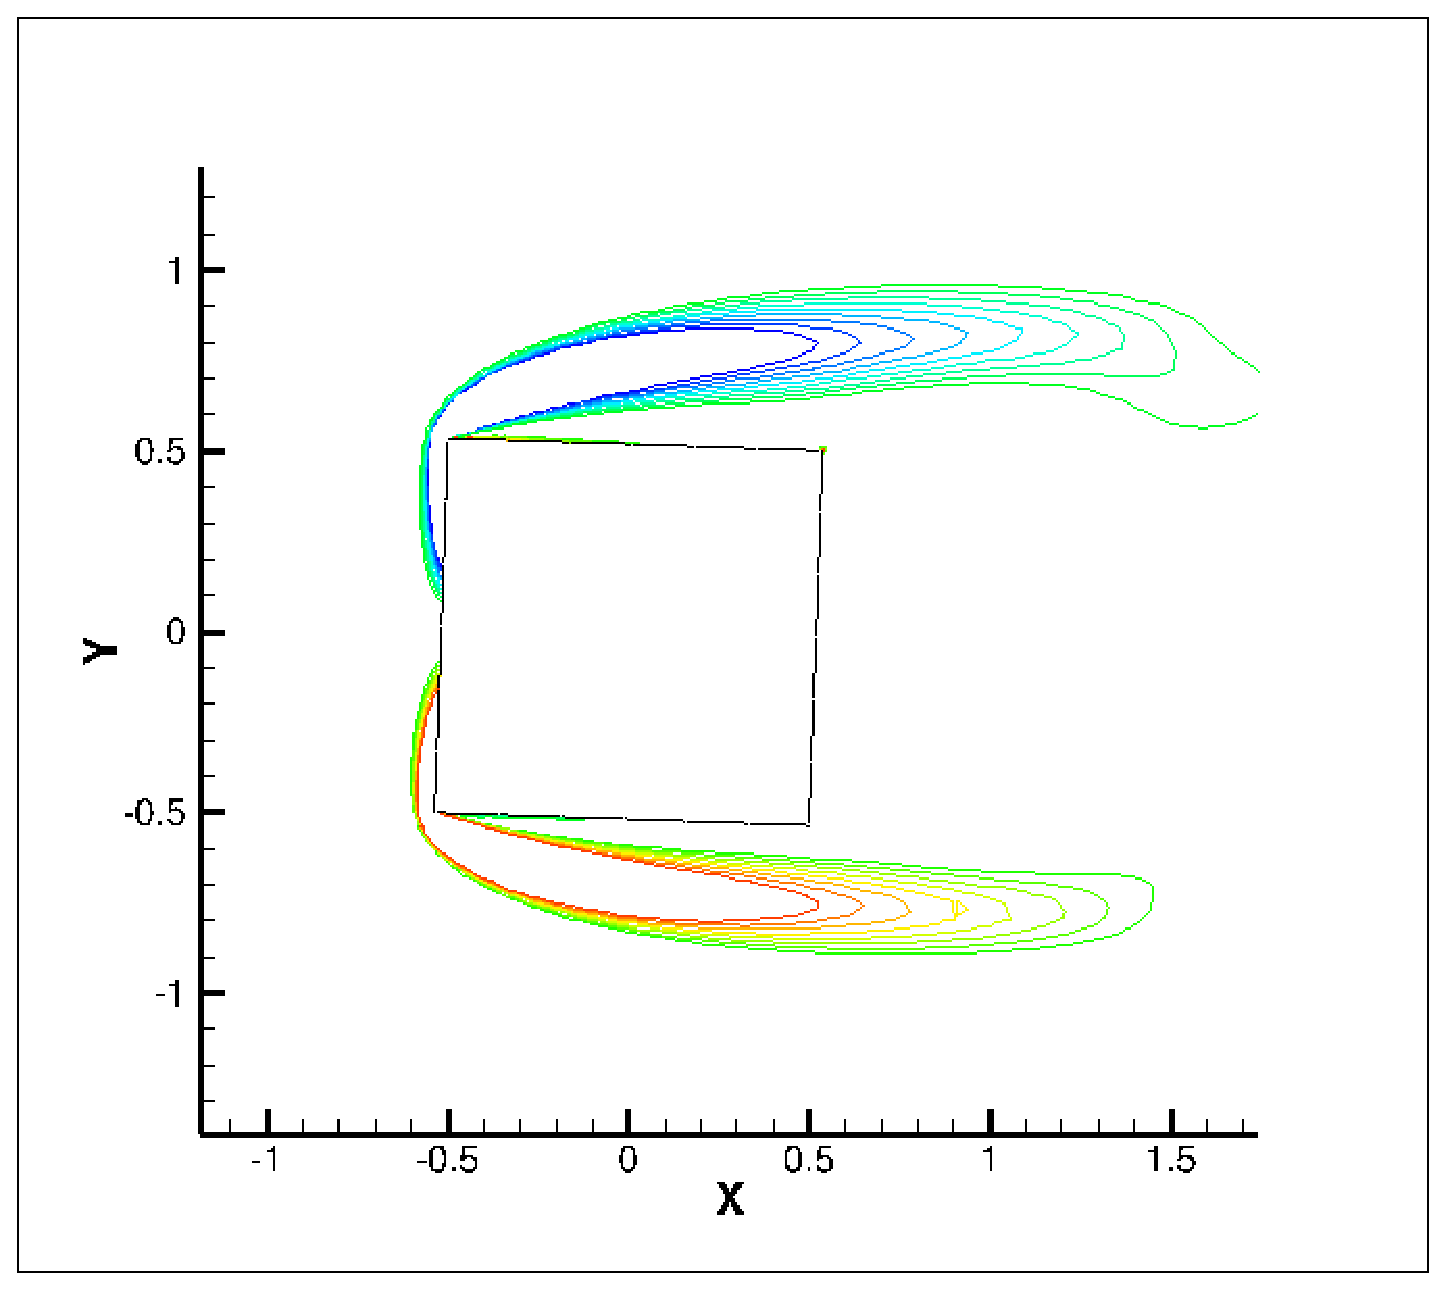
\includegraphics[width=0.33\unitlength]{./chapter-literature-revirw/fnp/square-2.eps}}
    \put(0.335,0.76){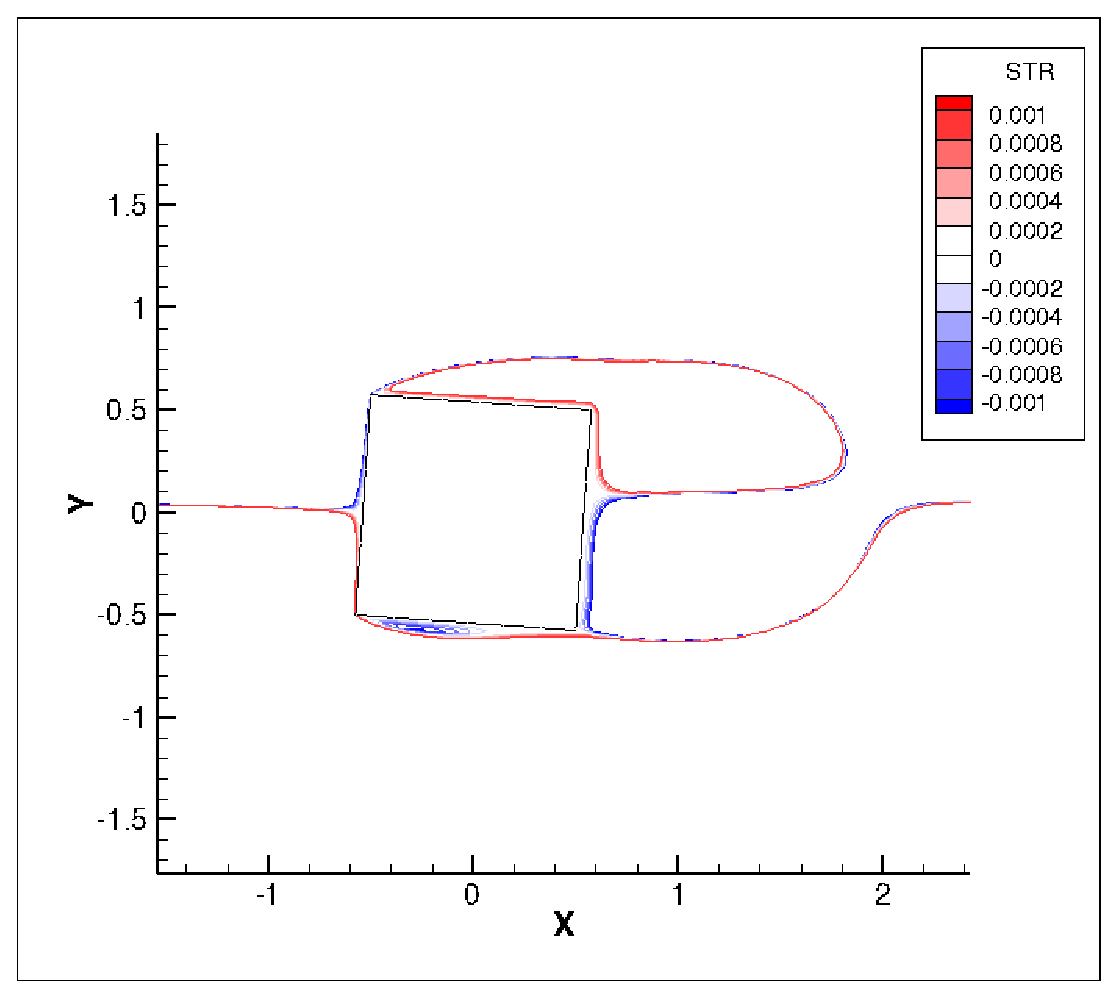
\includegraphics[width=0.33\unitlength]{./chapter-literature-revirw/fnp/square-4.eps}}
    \put(0.68,0.76){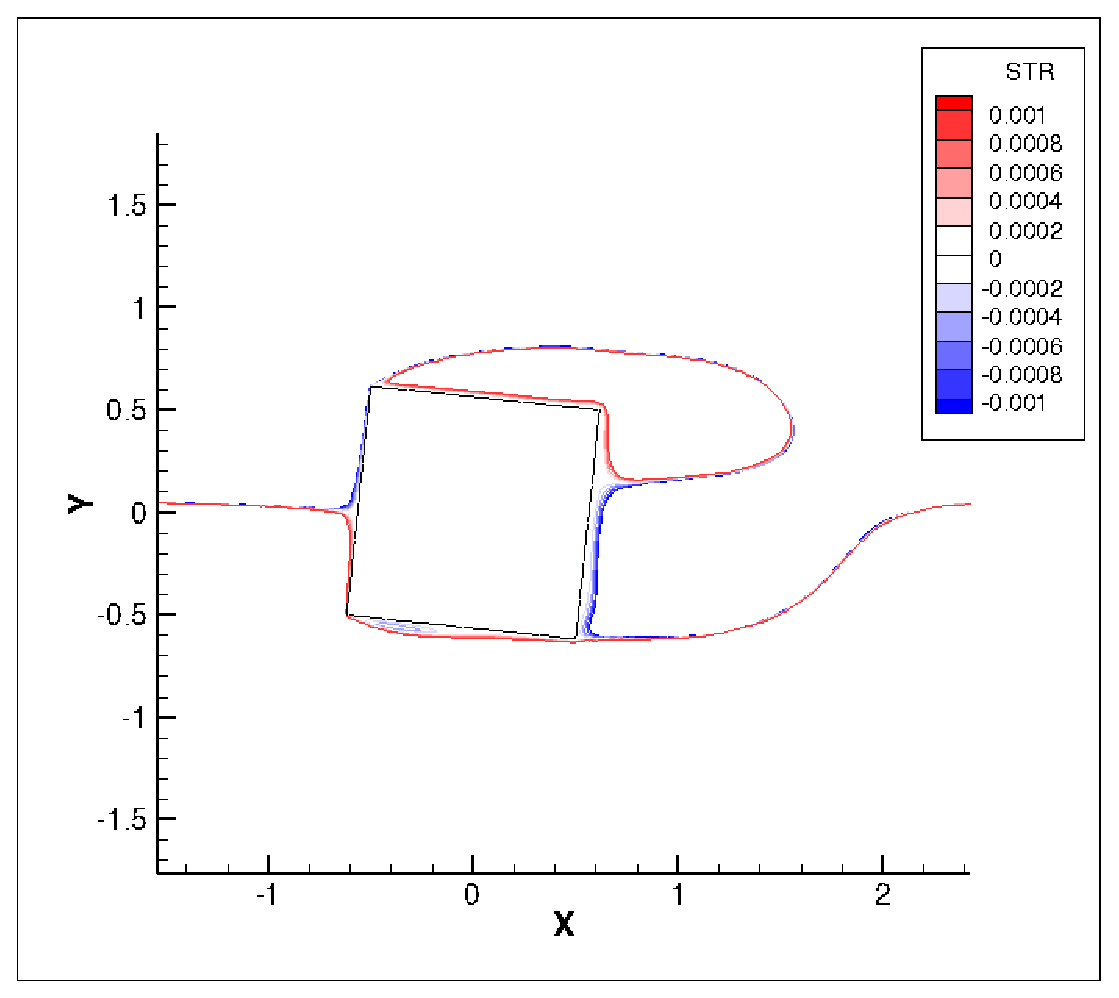
\includegraphics[width=0.33\unitlength]{.//chapter-literature-revirw/fnp/square-6.eps}}

   
    
    \put(0.0,0.735){(a)}    
    \put(0.34,0.735){(b)}
    \put(0.685,0.735){(c)}
  
  \end{picture}
}
  \caption{}
  \label{fig:shear_layers}
\end{figure}







In order to carry out an optimisation study on the fluid dynamics portion of the system, it is essential to study underlying fluid mechanics for galloping. It has been already established by \cite{Parkinson1964} that the instantaneous lift is the input of the system. Therefore it is essential to have an understanding on how exactly this lift occur. According to \cite{Parkinson1989},\cite{Luo1994} the lift force is created by the secondary flow of the two shear layers of either side of the body which creates an unbalanced pressure distribution on the afterbody (Fig.\ref{fig:shear_layers}). If a square cross section is taken as an example, when the body have a transverse $\dot{y}$, the relative velocity causes an instantaneous angle of attack which makes one shear layer lies closer to the body than the other. Therefore the shear layer near the body creates a pressure imbalance by creating a higher suction on the wall of the body on the adjacent side than the suction caused by the shear layer on the opposite side on its adjacent side of the body. The lift force become its maximum when the shear layer closer to the body reattaches at the trailing edge. As the angle of attack is further increased, the separated shear layer in the opposite side of the body (which was initially away from the body) shrinks therefore the pressure difference decreases which results a decrease in the lift force. This explanation was validated by \cite{Luo1994} by conducting flow visualisation experimentally.

Therefore two parameters could be identified which governs the lift 

\begin{itemize}
\item The characteristics of the afterbody
\item Shear layer separation
\item Shear layer reattachment 

\end{itemize}
 %\begin{figure}
  \centering
\fbox{
  \setlength{\unitlength}{\textwidth}
  \begin{picture}(0.6,0.5)

  
    % % %90
      \put(-0.1,0){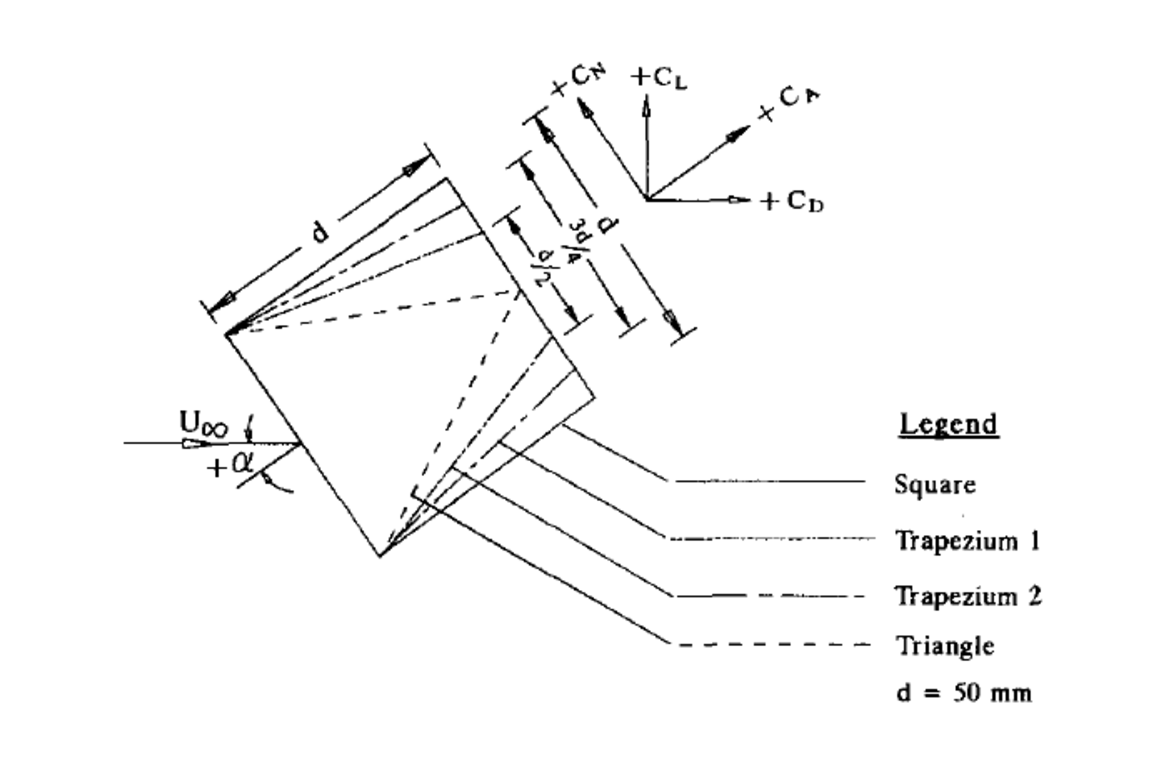
\includegraphics[width=0.75\unitlength]{./fnp/sketch-1.eps}}
     
% 	\put(0.02,0.93){ \large $C_y$} 	
%% 	\put(0.56,1.02){ $\theta$}
% 	
%        \put(0.25,0.8){ $\theta$} 	
%        \put(0.75,0.8){ $\theta$}
%        
%        \put(0.105,1.01){(a)}
%        \put(0.565,1.01){(b)}
     \end{picture}

 }
 \caption{Cross sectional shape considerd in in \cite{Luo2003}}
    \label{fig:lift_curves}
\end{figure}
.
\cite{Luo1994} have done some interesting studies on the lift characteristics on trapezoidal bodies. Which essentially the top and bottom sides of a square were tapered away systematically until it becomes triangle. According to the data presented \cite{Luo1994} the highest lift is produced by the triangle. However, the maximum lift occur at a very large angle of attack ($\theta\approx 34^0 $) compared to a square cross section ($\theta\approx 12^0 $).

\subsubsection{Optimising the cross sectional shape}
According to the literature survey done so far, investigations have been carried out only on cross sections with basic shapes. 

\begin{itemize}
\item{Square}
\item{Triangle}
\item{Trapezium}
\end{itemize}
   
Our hypothesis is that the cross section could be further optimised to get a higher power output by incorporating a complex shape which is a combination of the basic shapes. The current suggestion is that to analyse the characteristics of a hybrid shape of square and triangle. The idea is to delay the shear layer reattachment by tapering away the afterbody of the square cross section. This may result in having a larger band of induced angles where the forcing is substantially high. This will eventually then lead to a higher mean power output.

\input{./figures/proposed_sketch}





\begin{itemize}
\item{The stationary $c_y$ data of basic cross sections (i.e square, triangle and trapezium) will be obtained using DNS simulations at laminar flow. The data will be compared with existing literature. The time averaged pressure fields will be obtained in order to analyse the behaviour of the shear layers.}
\item{The stationary data of the complex shape shown in Fig.\ref{fig:complex_shape} will be obtained together with the time average pressure fields where the behaviour of the shear layers could be analysed.}
\item{Based on the initial results an optimisation study will be carried out by changing $\frac{d}{l}$. The quasi-steady model will be used to obtain the power output.}
\item{FSI simulations will be carried out and the power output will be compared with the data obtained using quasi-steady model.}
\end{itemize}  




%\begin{figure}[h]
%\centering
%\includegraphics[width=\textwidth]{./Gantt}
%\caption{Revised Gantt Chart}
%\label{fig:Gantt}
%\end{figure}


%\section{Difficulties and challenges} 
%%
%%\begin{enumerate}
%%      
%%\end{enumerate}
\clearpage
\bibliography{../bibtex/MCR}
\bibliographystyle{agsm}
\cleardoublepage
\appendix
\begin{center}
\section*{\LARGE Appendix 1}
\addcontentsline{toc}{section}{Appendix 1} 
\end{center}
Proposed table of contents of the final PhD thesis:
\begin{enumerate}
\item Preliminary remarks 
\item A review of literature
\begin{enumerate}[i]
\item Introduction
\item Flow induced vibrations 
\item Flow induced vibrations as a mechanism of energy harvesting
\item Aeroelastic galloping
\item Behaviour of shear layer 
\end{enumerate}
\item Methodology and validation
\begin{enumerate}[i]
\item Introduction
\item Governing equations and quasi-steady state model 
\item Numerical methods and boundary conditions 
\item The governing equations for the DNS method: Naiver-Stokes and continuity  
\item Discretisation  
\item Integration of substep equation 
\item Boundary conditions 
\item Spectral element method
\item Convergence and validation studies 
\item Summary
\end{enumerate}
\item Power analysis for high and low Reynolds numbers
\begin{enumerate}[i]
\item Introduction 
\item Stationary data 
\item Natural frequency 
\item Damping constant 
\item Mass ratio
\item FSI validation 
\item Summary 
\end{enumerate}

\item Optimisation of the cross sectional shape 
\begin{enumerate}[i]
\item Introduction 
\item Stationary data of basic shapes  
\item Stationary data of the hybrid cross section
\item Flow analysis  
\item Optimisation of the hybrid cross section 
\item Power analysis 
\item FSI validation
\item Summary 
\end{enumerate}

\item Conclusion
%\begin{enumerate}[i]
%\item Introduction
%\item Summary of the work
%\item Future directions
%\end{enumerate}
\end{enumerate}
\vspace{5cm}
\section*{\LARGE Appendix 2}
\addcontentsline{toc}{section}{Appendix 2}

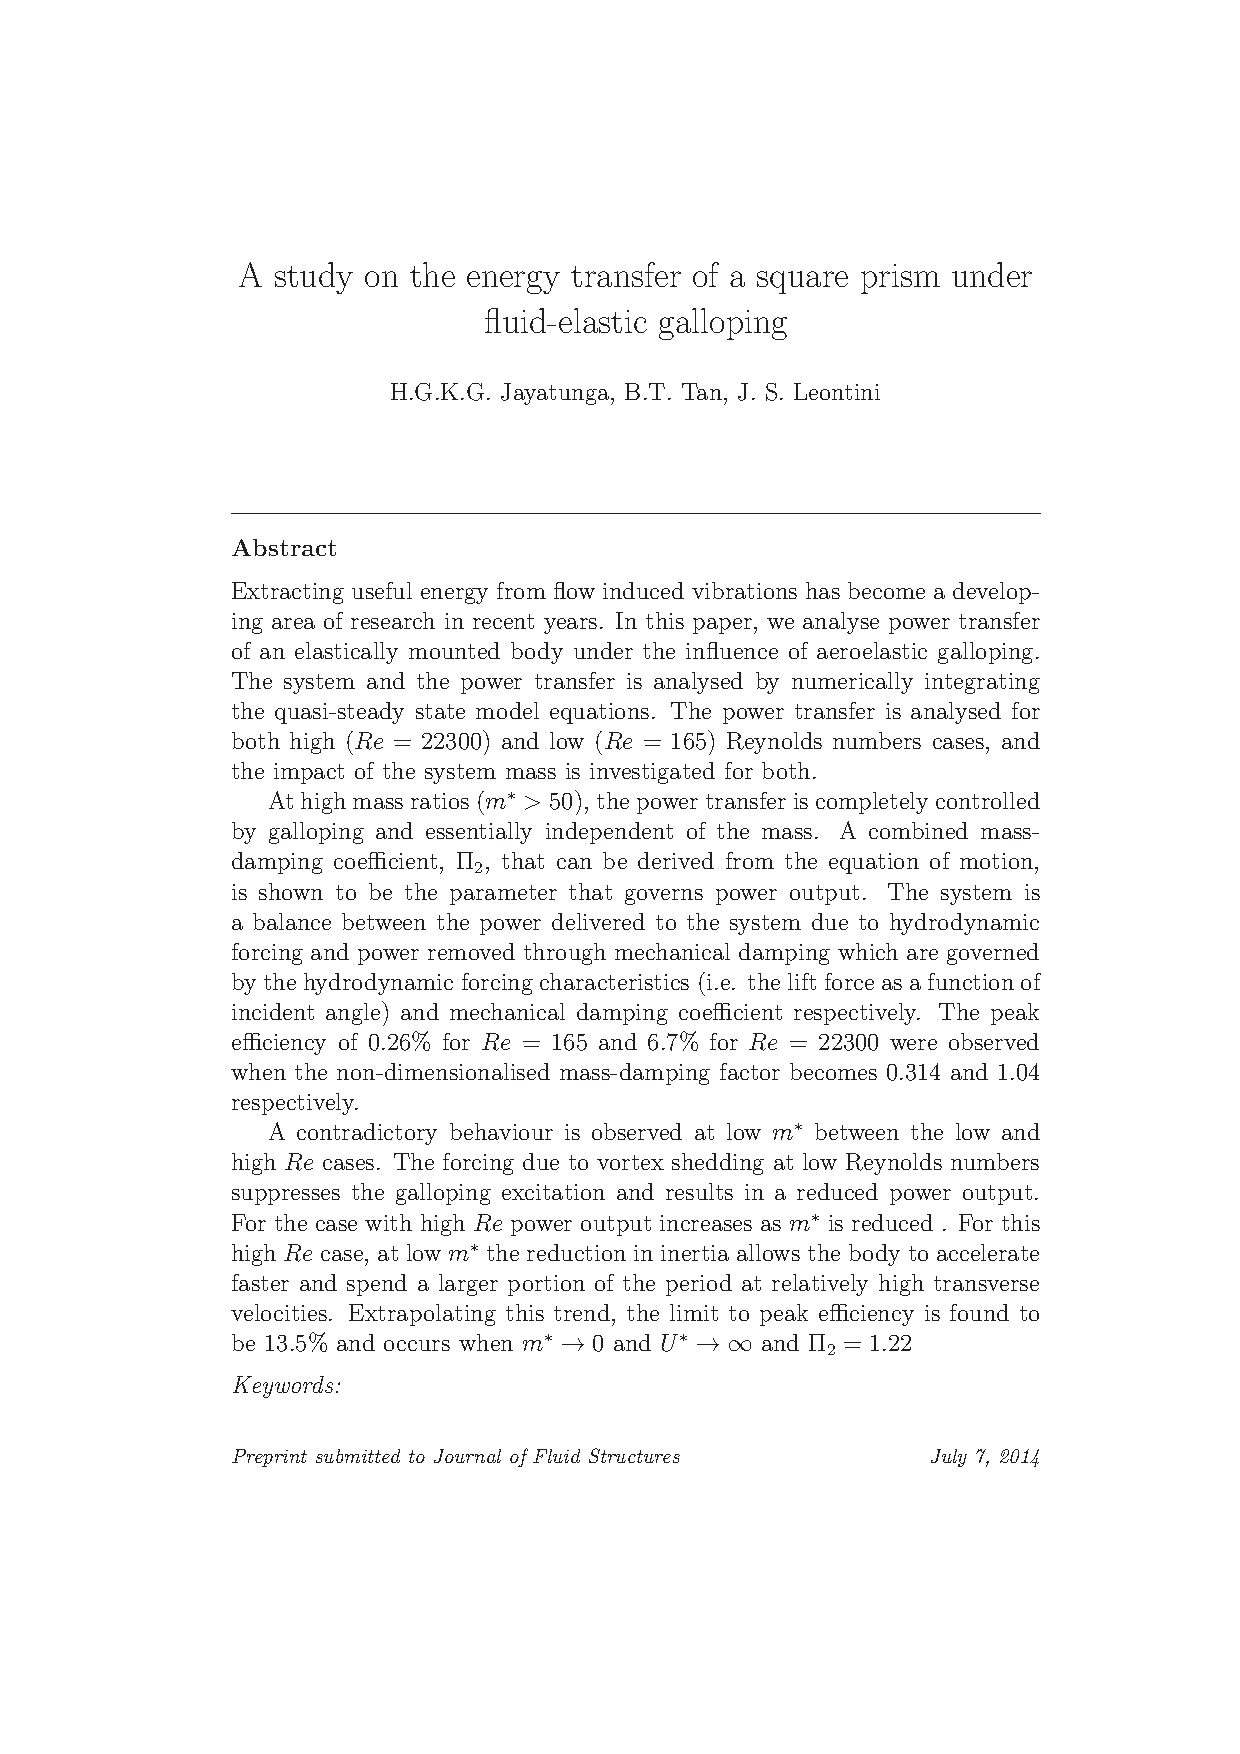
\includepdf[pages=1-18]{../paper/main/elsarticle-template-harv.pdf}

\end{document}